% Figure 1 — SAAC-JEPA architecture (Meta / I-JEPA visual language)
\documentclass[tikz,border=6pt]{standalone}
% Meta AI / FAIR figure style (I-JEPA / V-JEPA visual language)
% White background, soft pastel rounded blocks, thin borders, sans-serif,
% dashed arrows for EMA / stop-gradient, minimal ink.
\usepackage{amsmath,amssymb}
\usepackage[scaled]{helvet}
\renewcommand{\familydefault}{\sfdefault}
\usepackage{tikz}
\usetikzlibrary{arrows.meta,positioning,fit,calc,backgrounds}

% --- FAIR-like palette -------------------------------------------------------
\definecolor{mblue}{HTML}{BDD7EE}   \definecolor{mblueL}{HTML}{2E75B6}  % context / online encoder
\definecolor{mpink}{HTML}{F8CBAD}   \definecolor{mpinkL}{HTML}{ED7D31}  % target (EMA) encoder
\definecolor{mgreen}{HTML}{C6E0B4}  \definecolor{mgreenL}{HTML}{548235} % predictor
\definecolor{myell}{HTML}{FFE699}   \definecolor{myellL}{HTML}{BF9000}  % actions / conditioning
\definecolor{mgray}{HTML}{F2F2F2}   \definecolor{mgrayL}{HTML}{7F7F7F}  % latents / neutral
\definecolor{mred}{HTML}{F4B8B8}    \definecolor{mredL}{HTML}{C00000}   % loss / dead controls
\definecolor{ink}{HTML}{3B3B3B}

\tikzset{
  every node/.style={font=\sffamily},
  blk/.style={rounded corners=7pt, line width=0.7pt, minimum height=9mm,
              inner xsep=3mm, inner ysep=2mm, align=center, font=\sffamily\small},
  enc/.style ={blk, fill=mblue,  draw=mblueL},
  tgt/.style ={blk, fill=mpink,  draw=mpinkL},
  prd/.style ={blk, fill=mgreen, draw=mgreenL},
  act/.style ={blk, fill=myell,  draw=myellL},
  lat/.style ={blk, fill=mgray,  draw=mgrayL},
  los/.style ={circle, fill=mred, draw=mredL, line width=0.7pt, minimum size=7.5mm,
               font=\sffamily\small, inner sep=0pt},
  lbl/.style ={font=\sffamily\footnotesize, text=ink},
  sub/.style ={font=\sffamily\scriptsize, text=mgrayL},
  ar/.style  ={-{Latex[length=2.4mm]}, line width=0.8pt, draw=ink},
  ema/.style ={-{Latex[length=2.4mm]}, line width=0.8pt, draw=mpinkL, dashed},
  sg/.style  ={ar, postaction={decorate}},  % stop-gradient: annotate with // manually
  cell/.style={draw=mgrayL, line width=0.4pt, minimum size=3.2mm, inner sep=0pt},
  cellm/.style={cell, fill=mblue},          % visible patch
  cellx/.style={cell, fill=mgray},          % masked patch
}
% stop-gradient tick: \sgmark{point}
\newcommand{\sgmark}[1]{\node[rotate=65, font=\footnotesize\bfseries, text=ink] at (#1) {/\!/};}

\begin{document}
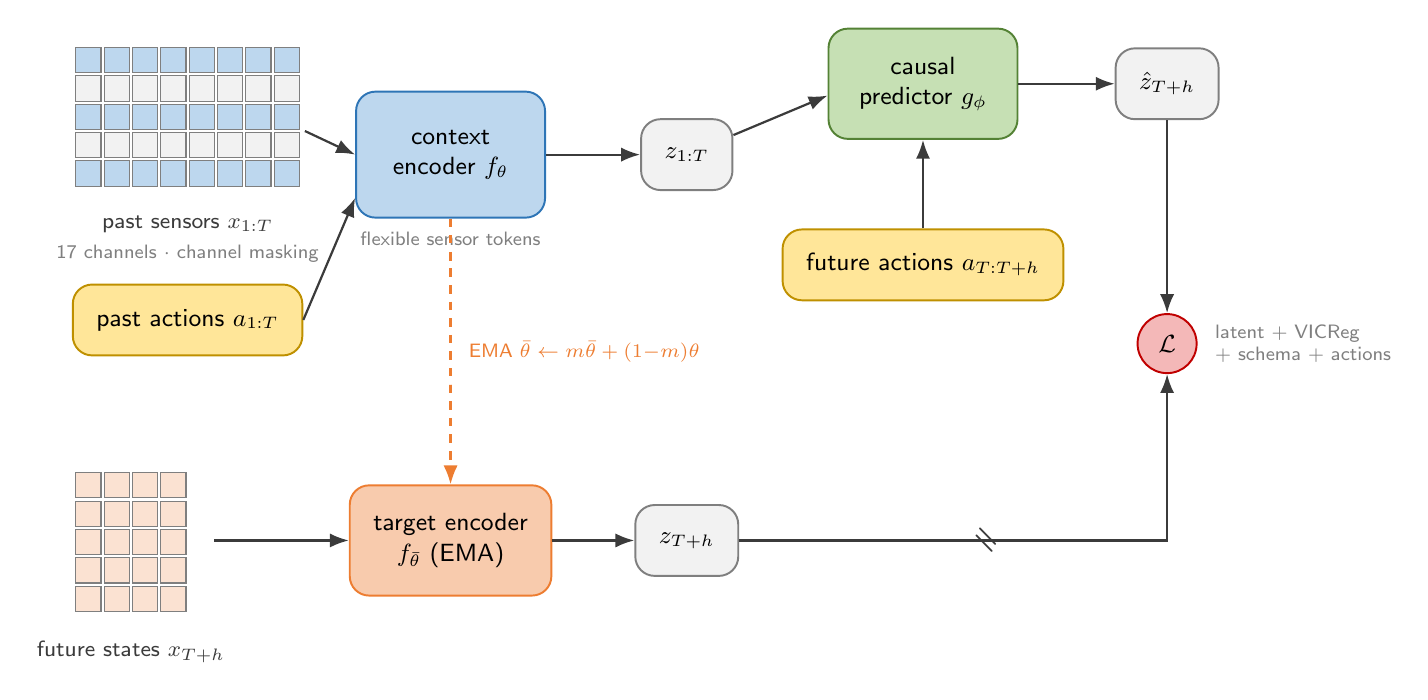
\begin{tikzpicture}[node distance=9mm]

% ---------------- inputs: sensor grid (some channels masked) ----------------
\begin{scope}[shift={(0,0)}]
  \foreach \t [count=\i from 0] in {0,...,7}{
    \foreach \c [count=\j from 0] in {0,...,4}{
      \pgfmathparse{(\j==1 || \j==3) ? 1 : 0}
      \ifnum\pgfmathresult>0
        \node[cellx] at (0.36*\i, -0.36*\j) {};
      \else
        \node[cellm] at (0.36*\i, -0.36*\j) {};
      \fi
    }
  }
  \node[lbl, anchor=north] at (1.26,-1.85) {past sensors $x_{1:T}$};
  \node[sub, anchor=north] at (1.26,-2.22) {17 channels $\cdot$ channel masking};
\end{scope}

% actions
\node[act, minimum width=26mm] (pact) at (1.26,-3.3) {past actions $a_{1:T}$};

% ---------------- context encoder -------------------------------------------
\node[enc, minimum width=24mm, minimum height=16mm] (ctx) at (4.6,-1.2)
  {context\\encoder $f_\theta$};
\node[sub, below=0.5mm of ctx] {flexible sensor tokens};

% latent
\node[lat] (z) at (7.6,-1.2) {$z_{1:T}$};

% ---------------- predictor ---------------------------------------------------
\node[prd, minimum width=24mm, minimum height=14mm] (pred) at (10.6,-0.3)
  {causal\\predictor $g_\phi$};
\node[act, minimum width=24mm] (fact) at (10.6,-2.6) {future actions $a_{T:T+h}$};

% predicted latents
\node[lat] (zhat) at (13.7,-0.3) {$\hat z_{T+h}$};

% ---------------- target branch (EMA) ----------------------------------------
\begin{scope}[shift={(0,-5.4)}]
  \foreach \t [count=\i from 0] in {0,...,3}{
    \foreach \c [count=\j from 0] in {0,...,4}{
      \node[cellm, fill=mpink!55] at (0.36*\i, -0.36*\j) {};
    }
  }
  \node[lbl, anchor=north] at (0.54,-1.85) {future states $x_{T+h}$};
\end{scope}

\node[tgt, minimum width=24mm, minimum height=14mm] (te) at (4.6,-6.1)
  {target encoder\\$f_{\bar\theta}$ (EMA)};
\node[lat] (zt) at (7.6,-6.1) {$z_{T+h}$};

% ---------------- loss --------------------------------------------------------
\node[los] (loss) at (13.7,-3.6) {$\mathcal{L}$};
\node[sub, right=1mm of loss, align=left]
  {latent + VICReg\\ + schema + actions};

% ---------------- arrows ------------------------------------------------------
\draw[ar] (2.75,-0.9) -- (ctx.west |- ctx.center) node[midway, above, sub] {};
\draw[ar] (pact.east) -- ($(ctx.west)+(0,-0.55)$);
\draw[ar] (ctx) -- (z);
\draw[ar] (z) -- ($(pred.west)+(0,-0.15)$);
\draw[ar] (fact.north) -- ($(pred.south)+(0,0)$);
\draw[ar] (pred) -- (zhat);
\draw[ar] (1.6,-6.1) -- (te.west);
\draw[ar] (te) -- (zt);
\draw[ar] (zhat) -- (loss);
\draw[ar] (zt.east) -| (loss.south);
\sgmark{11.4,-6.1}

% EMA dashed link
\draw[ema] (ctx.south) to[out=-90,in=90] node[midway, right=1mm, sub, text=mpinkL]
  {EMA $\bar\theta \leftarrow m\bar\theta + (1{-}m)\theta$} (te.north);

\end{tikzpicture}
\end{document}
